\documentclass[a4paper]{article}
\usepackage[utf8]{inputenc}
\usepackage[slovene]{babel}
\usepackage{graphicx}
\usepackage{hyperref}
\usepackage[nottoc]{tocbibind}
\usepackage{minted}
\usepackage{listings}
\usepackage{caption}
\usepackage{subcaption}
\usepackage{amsmath}
\usepackage{ dsfont }
\usepackage{siunitx}
\usepackage{multimedia}
\usepackage[table,xcdraw]{xcolor}
\setlength\parindent{0pt}

\definecolor{codegreen}{rgb}{0,0.6,0}
\definecolor{codegray}{rgb}{0.5,0.5,0.5}
\definecolor{codepurple}{rgb}{0.58,0,0.82}
\definecolor{backcolour}{rgb}{0.95,0.95,0.92}
\newcommand{\ddd}{\mathrm{d}}
\newcommand\myworries[1]{\textcolor{red}{#1}}
\newcommand{\Dd}[3][{}]{\frac{\ddd^{#1} #2}{\ddd #3^{#1}}}
\newcommand{\Pd}[3][{}]{\frac{\partial^{#1} #2}{\partial #3^{#1}}}

\lstdefinestyle{mystyle}{
    backgroundcolor=\color{backcolour},   
    commentstyle=\color{codegreen},
    keywordstyle=\color{magenta},
    numberstyle=\tiny\color{codegray},
    stringstyle=\color{codepurple},
    basicstyle=\ttfamily\footnotesize,
    breakatwhitespace=false,         
    breaklines=true,                 
    captionpos=b,                    
    keepspaces=true,                 
    numbers=left,                    
    numbersep=5pt,                  
    showspaces=false,                
    showstringspaces=false,
    showtabs=false,                  
    tabsize=2
}

\lstset{style=mystyle}

\begin{document}
\begin{titlepage}
    \begin{center}
        
\includegraphics[]{logo.png}
        \vspace*{3cm}
        
        \Huge
        \textbf{Spektralne metode za začetne probleme PDE}
        
        \vspace{0.5cm}
        \large
        9. naloga pri Matematično-fizikalnem praktikumu

        \vspace{4.5cm}
        
        \textbf{Avtor:} Marko Urbanč (28191096)\ \\
        \textbf{Predavatelj:} prof. dr. Borut Paul Kerševan\ \\
        
        \vspace{2.8cm}
        
        \large
        1.9.2023
    \end{center}
\end{titlepage}
\tableofcontents
\newpage
\section{Uvod}
Parcialne diferencialne enačbe (PDE) lahko rešujemo na več različnih načinov.
Glavna razlika je v tem, kako diskretiziramo prostor in čas. V tej nalogi bomo 
reševali PDE z spektralnimi metodami.(Drugo možnost; diferenčne metode, bomo 
obravnavali v naslednji nalogi.) Pri spektralnih metodah diskretiziramo prostor s
tem, začetni pogoj izrazimo z nekim naborom baznih funkcij in nato iščemo rešitev
tako, da računamo, kako se koeficienti teh baznih funkcij spreminjajo s časom.
V tej nalogi bomo preizkusili reševanje preko Fourierove metode in metode končnih
elementov s kubičnimi B-zlepki.\\

\subsection{Fourierova metoda}
Fizikalno gledano rešujemo enodimenzionalno toplotno enačbo, torej difuzijsko enačbo,
v homogeni neskončni plasti, s končno debelino $a$, brez izvirov in ponorov toplote.

\begin{equation}
    D\Pd[2]{T}{x} = \Pd{T}{t}\quad 0\leq x \leq a,\quad D=\frac{\lambda}{\rho c}\>.
    \label{eq:1}
\end{equation}

Če Temperaturo $T(x, y)$ izrazimo kot Fourierovo vrsto dobimo

\begin{equation}
    T(x, t) = \sum_{k=0}^{N-1}{\hat{T}_k(t)\exp{\left(\frac{-2\pi i k x}{a}\right)}}\>. 
\end{equation}

Torej se PDE (\ref{eq:1}) zdaj zapiše kot

\begin{equation}
    \sum_{k=0}^{N-1}{\left(-\frac{4\pi^2 k^2 D}{a^2}\right)\hat{T}_k(t)\exp{\left(-\frac{2\pi i k x}{a}\right)}} = 
    \sum_{k=0}^{N-1}{\left(\frac{\ddd \hat{T}_k(t)}{\ddd t}\right)\exp{\left(-\frac{2\pi i k x}{a}\right)}}\>.
\end{equation}

Torej se naša naloga prevede na iskanje koeficientov $\hat{T}_k(t)$, ki jih dobimo preko
\textbf{evolucijske enačbe}
\begin{equation}
    \frac{\ddd \hat{T}_k(t)}{\ddd t} = -\frac{4\pi^2 k^2 D}{a^2}\hat{T}_k(t)\>.
    \label{eq:2}
\end{equation}

Pogosto se uporabi spektralno reprezentacijo za krajevni odvod, časovni korak pa naredimo
z neko ekspliticitno metodo. V našem primeru bomo uporabili \textbf{Eulerjevo metodo}.

\begin{equation}
    \hat{T}_k(t+k) = \hat{T}_k(t) + \frac{4\pi^2 k^2 D}{a^2}\hat{T}_k(t)k\>.
    \label{eq:3}
\end{equation}

Reprezentacijo $T(x, y)$ v običajnem prostoru dobimo z obratno Fourierovo transformacijo. Enačba
(\ref{eq:2}) ima analitično rešitev

\begin{equation}
    \hat{T}_k(t) = \hat{T}_k(0)\exp{\left(-\frac{4\pi^2 k^2 D}{a^2}t\right)}\>.
    \label{eq:4}
\end{equation}

To bo koristno za preverjanje numeričnih metod.\\
\subsection{Metoda končnih elementov}
Pri razvoju $T(x,y)$ nismo omejeni samo na trigonometrične funkcije. Lahko uporabimo tudi
poljubne druge funkcije. V našem primeru bomo uporabili kubične B-zlepke. To so funkcije
oblike

\begin{equation}
    B_{i, k}(x) = \frac{x-x_i}{x_{i+k}-x_i}B_{i, k-1}(x) + \frac{x_{i+k+1}-x}{x_{i+k+1}-x_{i+1}}B_{i+1, k-1}(x)\>.
\end{equation}

Začetni pogoj bomo izrazili kot linearno kombinacijo teh funkcij in nato iščemo rešitev
v obliki

\begin{equation}
    T(x, t) = \sum_{i=-1}^{N+1}{c_k(t)B_{i, 3}(x)}\>.
\end{equation}

Tako zasnujemo metodo končnih elementov, s kolokacijskim pogojem. To pomeni, da se začetni
pogoj mora ujemati z rešitvijo na nekem končnem številu točk. Podobno kot pri Fourierovi metodi
vstavimo razvoj v PDE in dobimo sistem enačb za koeficiente $\hat{T}_i(t)$

\begin{equation}
    \sum_{i=-1}^{N+1}{D c_k(t)B_{i, 3}(x)} = 
    \sum_{i=-1}^{N+1}{\left(\frac{\partial c_k(t)}{\partial t}\right)B_{i, 3}(x)}\>.
\end{equation}

Uporabimo lastnosti B-zlepkov in dobimo sistem diferencialnih enačb za koeficiente $c_k(t)$

\begin{equation}
    \dot{c}_{j-1}(t) + 4\dot{c}_{j}(t) + \dot{c}_{j+1}(t) = \frac{6D}{h^2}(c_{j-1}(t) - 2c_j(t) + c_{j+1}(t))\>,
\end{equation}

kjer je $h$ razdalja med točkami, ki smo jih izbrali za kolokacijski pogoj. Iz robnega pogoja pri $x=0$
ugotovimo, da je $c_{-1} = -4c_0-c_1$. Podobno iz robnega pogoja pri $x=a$ sledi $c_0 = C_N = 0$ in $c_{-1} = -c_1$
ter $c_{N-1} = -c_{N+1}$. Reševanje smo torej prevedli na reševanje matričnega sistema

\begin{equation}
    \mathbf{A} \frac{\ddd \vec{c}}{\ddd t} = \mathbf{B}\vec{c}\>,
\end{equation}

kjer je $\mathbf{A}$ tridiagonalna matrika z $4$ na diagonali in $1$ na pod in nad diagonalo

\begin{equation}
    \mathbf{A}=\begin{bmatrix}
        4 & 1 & 0 & \cdots & 0 & 0 & 0\\
        1 & 4 & 1 & \cdots & 0 & 0 & 0\\
        0 & 1 & 4 & \cdots & 0 & 0 & 0\\
        \vdots & \vdots & \vdots & \ddots & \vdots & \vdots & \vdots\\
        0 & 0 & 0 & \cdots & 4 & 1 & 0\\
        0 & 0 & 0 & \cdots & 1 & 4 & 1\\
        0 & 0 & 0 & \cdots & 0 & 1 & 4\\
    \end{bmatrix}\>,
\end{equation}

$\mathbf{B}$ tridiagonalna matrika z $-2$ na diagonali in $1$ na pod in nad diagonalo pomnožena z $6D/h^2$

\begin{equation}
    \mathbf{B}=\frac{6D}{h^2}\begin{bmatrix}
        -2 & 1 & 0 & \cdots & 0 & 0 & 0\\
        1 & -2 & 1 & \cdots & 0 & 0 & 0\\
        0 & 1 & -2 & \cdots & 0 & 0 & 0\\
        \vdots & \vdots & \vdots & \ddots & \vdots & \vdots & \vdots\\
        0 & 0 & 0 & \cdots & -2 & 1 & 0\\
        0 & 0 & 0 & \cdots & 1 & -2 & 1\\
        0 & 0 & 0 & \cdots & 0 & 1 & -2\\
    \end{bmatrix}\>,
\end{equation}

in $\vec{c}$ vektor koeficientov $c_k(t)$. Začetni pogoj za PDE je $T(x, 0) = f(x)$, torej je začetni približek
za kolokacijsko aproksimacijo

\begin{equation}
    \mathbf{A}\vec{c} = \vec{f}\>,
\end{equation}

kjer je $\vec{f}$ vektor $f(x_i)$. To zdaj rešujemo z neko eksplitično metodo. V našem primeru bomo uporabili
\textbf{Implicitno Eulerjevo metodo} zaradi njene stabilnosti. To pomeni, da za časovni korak $k$ velja

\begin{equation}
    \mathbf{A}\frac{\vec{c}_{k+1}-\vec{c}_k}{\Delta t} = \mathbf{B}\vec{c}_{k+1}\>.
\end{equation}

\section{Naloga}
Naloga od nas zahteva da v eni razsežnosti rešimo PDE (\ref{eq:1}) z začetnim pogojem
po plasti gaussovsko porazdeljene temperature

\begin{equation}
    T(x, 0) \propto \exp{\left(-\frac{(x-a)^2}{2\sigma^2}\right)}\>.
\end{equation}

Rešiti moramo za periodični robni pogoj $T(0, t) = T(a, t)$ in homogeni Dirichletov robni pogoj
$T(0, t) = T(a, t) = 0$ po Fourierevi metodi. Kolokacijsko metodo nato uporabi za reševanje
PDE z nehomogenim Dirichletovim robnim pogojem $T(0, t) = T(a, t) = 0$ in istim začetnim pogojem.
in primerjamo obe metodi.\\

\section{Opis reševanja}
Po (pre)dolgem premoru sem se lotil reševanja naloge, spet na tradicionalen način, torej z uporabo 
Pythona in knjižnic \texttt{numpy} in \texttt{scipy}. Za risanje grafov sem uporabil knjižnico
\texttt{matplotlib}. Zdaj imam tudi nekaj trikov v rokavu, ki sem jih uspel na hitro preizkusiti.\\

Po tem ko sem se lotil reševanja naloge sem ugotovil, da je bil moj prvoten pristop (opisan v 
datoteki \texttt{src.py}) popolnoma nepraktičen in napačen. Lotil sem se reševanja na novo in sicer
z bolj sistematičnim pristopom. Za obe metodi sem napisal razred, ki vsebuje vse potrebne funkcije
za reševanje. Poglejmo si to podrobneje.\\

\subsection{SpectralSolver}
Razred \texttt{SpectralSolver} je namenjen reševanju PDE po Fourierovi metodi. V konstruktorju
razreda se inicializirajo vsi potrebni parametri, ki jih potrebujemo za reševanje. To so 
difuzijska konstanta $D$, debelina plasti $a$, število točk v prostoru $N$, začetni pogoj $f(x)$ in
niz časov za katere računamo rešitev. Od tu naprej uporabnik pokliče eno od metod za reševanje
PDE. Torej ali \texttt{solve\_Analytically()} ali \texttt{solve\_Numerically()}. Prva metoda uporablja
analitično rešitev, ki je podana z enačbo (\ref{eq:4}). Druga metoda pa uporablja \\
\texttt{scipy.integrate.odeint()} za reševanje sistema enačb (\ref{eq:2}).\\

Po opravljenem reševanju vsebuje razred tudi vse metode za izris raznih grafov. Zna risati te 
zvezne line plot-e, ki jih uporabljam za risanje temperaturnega profila v odvisnosti od časa. Zna
risati "Heatmap" grafe in tudi animacije, ki jih žal ni smiselno dati v statično poročilo. Obstajajo
tudi eksperimentalne metode za neke hexbin grafe in 3D grafe, ki jih na koncu nisem uporabil, ampak
obstajajo pa, če bi jih kdo rad uporabil.\\

\subsection{ColocationSolver}
Podobno, obstaja razred \texttt{ColocationSolver}, ki je namenjen reševanju PDE po metodi končnih
elementov. Tudi ta razred vsebuje vse potrebne parametre za reševanje, ki se incializira v 
konstruktorju. Parametri so enaki kot pri prejšnjem razredu. Razred ima tudi dve metode za
reševanje PDE. Prva je \texttt{solve\_Properly()}, ki uporablja \texttt{scipy.linalg.solve\_banded()},
da reši sistem enačb. Druga metoda je \texttt{solve\_Manually()}, ki reši sistem enačb z Thomasovim
algoritmom. Ta metoda je načeloma precej hitrejša. Razred vsebuje tudi metode za risanje grafov, ki so
enake kot pri prejšnjem razredu.\\


\subsection{MPI\_Node}
Oče mi je dal nasvet, da naj poskusim pri zaključku 1. stopnje faksa biti pragmatičen in se ne ukvarjati
z nekimi nepotrebnimi stvarmi. No jaz sem pač nekoliko glup in imam zdaj precej časovno stisko, kako
naj bi uspel vse končati... ampak imam pa paralelizirane metode preko MPI-ja heh. (Pri tržni raziskavi
te naloge se je izkazalo, da so tudi vsi ostali istega mnenja kot moj oče.)\\

Razred \texttt{MPI\_Node} je namenjen paralelizaciji reševanja PDE. V konstruktorju se inicializira
MPI komunikator, ki ga uporabljamo za komunikacijo med procesi. V osnovi je to samo ovoj (angl. wrapper)
okoli prejšnjih dveh razredov. Vsebuje metode za delitev intervalov podatkov in za pošiljanje podatkov
med procesi. Vsebuje tudi metode za risanje grafov, ki so enake kot pri prejšnjih dveh razredih, le da jih
opravlja lahko samo "root" proces.\\

\subsection{GatherStatistics}
Zato da res pripeljem do konca idejo, da sem nepraktičen, sem napisal še en razred, pravzaprav še en ovoj okoli
\texttt{MPI\_Node}, ki je namenjen temu da zbira statistiko o času izvajanja. Želel sem dobiti značilne premice
v log-log skali, ki kažejo na uspešno paralelizacijo, ampak sem to le deloma uspel.\\

\section{Rezultati}
Sedaj pa končno rezultati. Ker žal nimam nobenih "grafov 3. reda", kompenziram za pomanjkanje s tem, da
so grafi divje pisani.\\

\subsection{Fourierova metoda}
\subsubsection{Periodični robni pogoji}
Najprej si poglejmo rezultate za periodične robne pogoje. Slike so rešene za mrežo točk $N=10000$ in difuzijsko
konstanto $D=1e-3$. Začetni pogoj je gaussovka z $\sigma=1$ in $a=5$, na intervalu $[0, 10]$. 
Začnimo z analitično rešitvijo. Na sliki \ref{fig:1}

\begin{figure}[H]
    \centering
        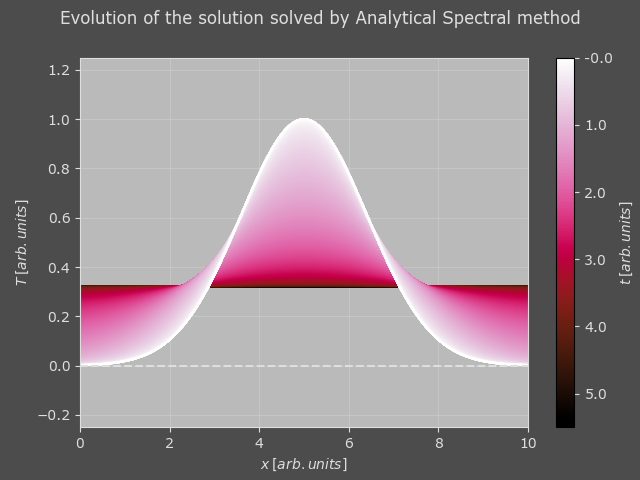
\includegraphics[width=\linewidth]{./images/S_Analytic_P.png}
        \caption{Analitična rešitev}
    \label{fig:1}
\end{figure}

\begin{figure}[H]
    \centering
        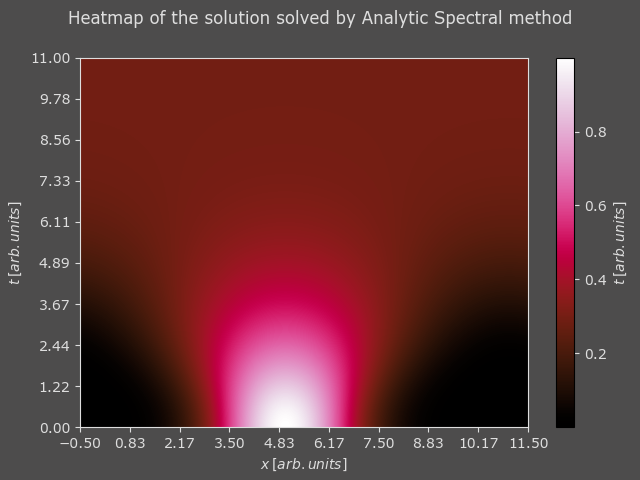
\includegraphics[width=\linewidth]{./images/S_Analytic_P_Heatmap.png}
        \caption{Še heatmap analitične rešitve}
    \label{fig:2}
\end{figure}

Kot pričakovano se temperaturna porazdelitev z časom razširi in zgladi. Zaradi periodičnih robnih pogojev
se temperatura ustali pri neki konstantni vrednosti okoli $0.36$ arbitrarnih enot. Super zdaj vemo proti 
čemu tekmujemo z numeričnimi metodami. Poglejmo si rezultate za \texttt{solve\_Numerically()} na sliki \ref{fig:3},
ki bodo seveda skočili na naslednjo stran (ampak je to vseeno boljše kot slike na koncu poročila).

\begin{figure}[H]
    \centering
        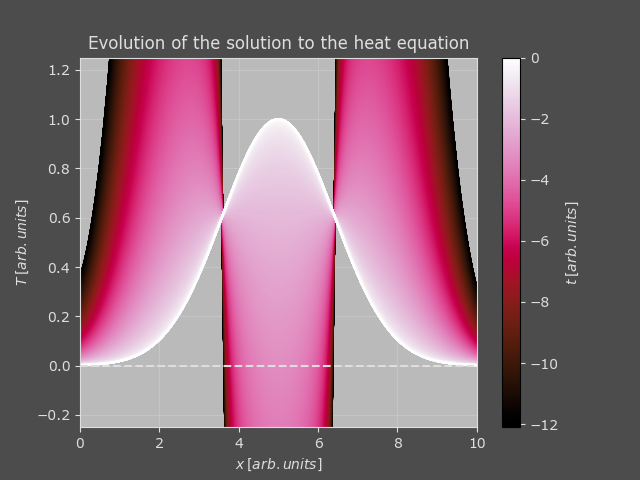
\includegraphics[width=\linewidth]{./images/S_Numeric_P.png}
        \caption{Numerična rešitev}
    \label{fig:3}
\end{figure}

\begin{figure}[H]
    \centering
        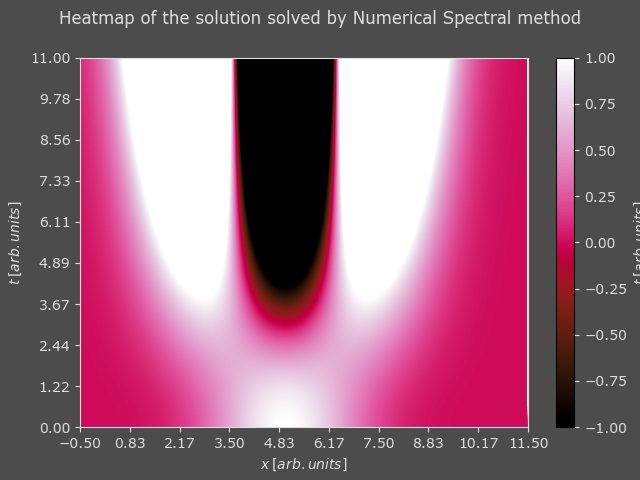
\includegraphics[width=\linewidth]{./images/S_Numeric_P_Heatmap.png}
        \caption{Še heatmap numerične rešitve}
    \label{fig:4}
\end{figure}

Kot vidimo, se numerična rešitev absolutno NE ujema z analitično in iskreno ne vem zakaj. Poleg vgrajenega
integratorja iz \texttt{scipy} sem poskusil tudi Runge-Kutta 8 integrator, ki sem ga napisal sam (guess kdo je
spet zapravil preveč časa na tem), Eulerjevo metodo, RK45 ipd. ampak tudi to ni pomagalo. I tried I suppose.

\subsubsection{Dirichletovi robni pogoji}
Zdaj pa poglejmo še rezultate za Dirichletove robne pogoje. Začetni pogoj je enak kot prej, ampak to le "v teoriji".
V resnici moramo narediti liho razširitev funkcije in intervala na katerem integriramo. Torej je začetni pogoj

\begin{equation}
    T(x, 0) \propto \exp{\left(-\frac{(x-a)^2}{2\sigma^2}\right)} - \exp{\left(-\frac{(x+a)^2}{2\sigma^2}\right)}\>.
\end{equation}

Rišemo še vedno za isti interval, le da smo zdaj s tem trikom dobili robni pogoj $T(0, t) = T(a, t) = 0$. Dobimo sliko
\ref{fig:5}.

\begin{figure}[H]
    \centering
        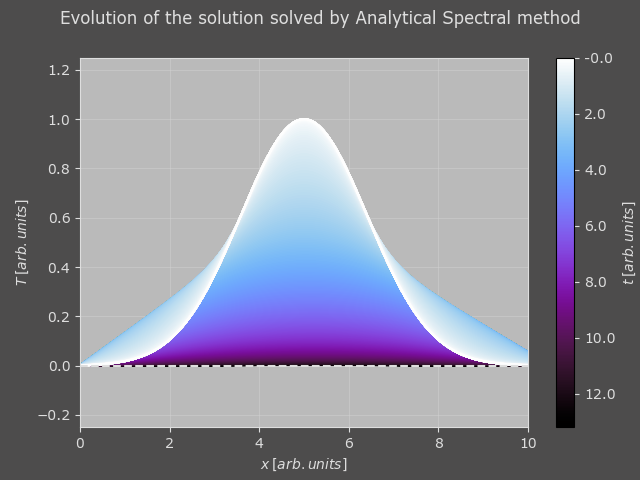
\includegraphics[width=\linewidth]{./images/S_Analytic_D.png}
        \caption{Analitična rešitev, pri Dirichletovih robnih pogojih}
    \label{fig:5}
\end{figure}

\begin{figure}[H]
    \centering
        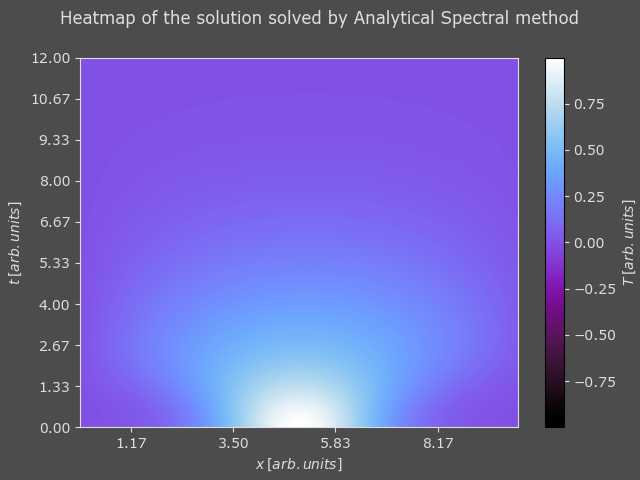
\includegraphics[width=\linewidth]{./images/S_Analytic_D_Heatmap.png}
        \caption{Še heatmap analitične rešitve, pri Dirichletovih robnih pogojih}
    \label{fig:6}
\end{figure}

\section{Komentarji in izboljšave}

\newpage
\bibliographystyle{unsrt}
\bibliography{sources}
\end{document}
